\documentclass[lesson_slides]{subfiles}
\usepackage{natbib}
\usepackage{graphicx}
% \graphicspath{ {./images/} }
\usepackage{enumerate}
\usepackage{pifont} % for ding
\usepackage{float} % keeps tables in the exact position they occupy in the code
\usepackage{xcolor} % text colour
\usepackage{gb4e} % leave last

\begin{document}
%%=-=-=-=-=-=-=-=-=-=-=-=-=-=-=-=-=-=-=-=-=-=-=-=-=-=-=-=-=-=-=-=-=-=-=-=-=-=-=-=
%   FRAME START   -=-=-=-=-=-=-=-=-=-=-=-=-=-=-=-=-=-=-=-=-=-=-=-=-=-=-=-=-=-=-=
\begin{frame}[c]{Activation of FocusP in French wh-questions}

    \transboxin<1>
    \transglitter<2>
    %\transwipe<3>
    In an earlier section, we saw that the parametrisation of FocusP can change crosslinguistically. \pause

    %\noindent \textbf{\textsc{variations in the activation of focusp}} 
    \begin{table}[H]
    \centering
        \begin{tabular}{|l|r|r|r|r|r|r|}
        \hline
         & Merge & Spell Out & Search & IM & Search\textsubscript{lex} & IM\textsubscript{lex} \\
        \hline
        Italian & 1 & 0 & 1 & 1 & 0 & 0 \\
        \hline
        Gungbe & 1 & 1 & 1 & 1 & 0 & 0 \\
        \hline
        German & 1 & 0 & 1 & 1 & 1 & 1 \\
        \hline
        \end{tabular}
    \caption{\label{tab:samp}Language variability in activating FocusP (\citealt{samo2019cartography}: 147 (10)).}
    \end{table}

\end{frame}
%   FRAME END   --==-=-=-=-=-=-=-=-=-=-=-=-=-=-=-=-=-=-=-=-=-=-=-=-=-=-=-=-=-=-=
%   FRAME START   -=-=-=-=-=-=-=-=-=-=-=-=-=-=-=-=-=-=-=-=-=-=-=-=-=-=-=-=-=-=-=
\begin{frame}[c]{Activation of FocusP in French wh-questions}

\begin{center}
    \bf{The parametrisation can change even language-internally!}
\end{center}

\end{frame}
%   FRAME END   --==-=-=-=-=-=-=-=-=-=-=-=-=-=-=-=-=-=-=-=-=-=-=-=-=-=-=-=-=-=-=
%   FRAME START   -=-=-=-=-=-=-=-=-=-=-=-=-=-=-=-=-=-=-=-=-=-=-=-=-=-=-=-=-=-=-=
\begin{frame}[c]{Activation of FocusP in French wh-questions}

    \transboxin<1>
    \transglitter<2>
    \transwipe<3>
    In French, we observe four possible configurations: \pause (question-formation strategies) \pause
    \begin{itemize}
        \item[\ding{227}] two ;
        \item[\ding{227}] ;
        \item[\ding{227}] ;
    \end{itemize}

\end{frame}
%   FRAME END   --==-=-=-=-=-=-=-=-=-=-=-=-=-=-=-=-=-=-=-=-=-=-=-=-=-=-=-=-=-=-=
%   FRAME START   -=-=-=-=-=-=-=-=-=-=-=-=-=-=-=-=-=-=-=-=-=-=-=-=-=-=-=-=-=-=-=
\begin{frame}[c]{Activation of FocusP in French wh-questions}

in situ: “Tu as vu qui?”

\end{frame}
%   FRAME END   --==-=-=-=-=-=-=-=-=-=-=-=-=-=-=-=-=-=-=-=-=-=-=-=-=-=-=-=-=-=-=
%   FRAME START   -=-=-=-=-=-=-=-=-=-=-=-=-=-=-=-=-=-=-=-=-=-=-=-=-=-=-=-=-=-=-=
\begin{frame}[c]{Combinations for French}

    \begin{center}
        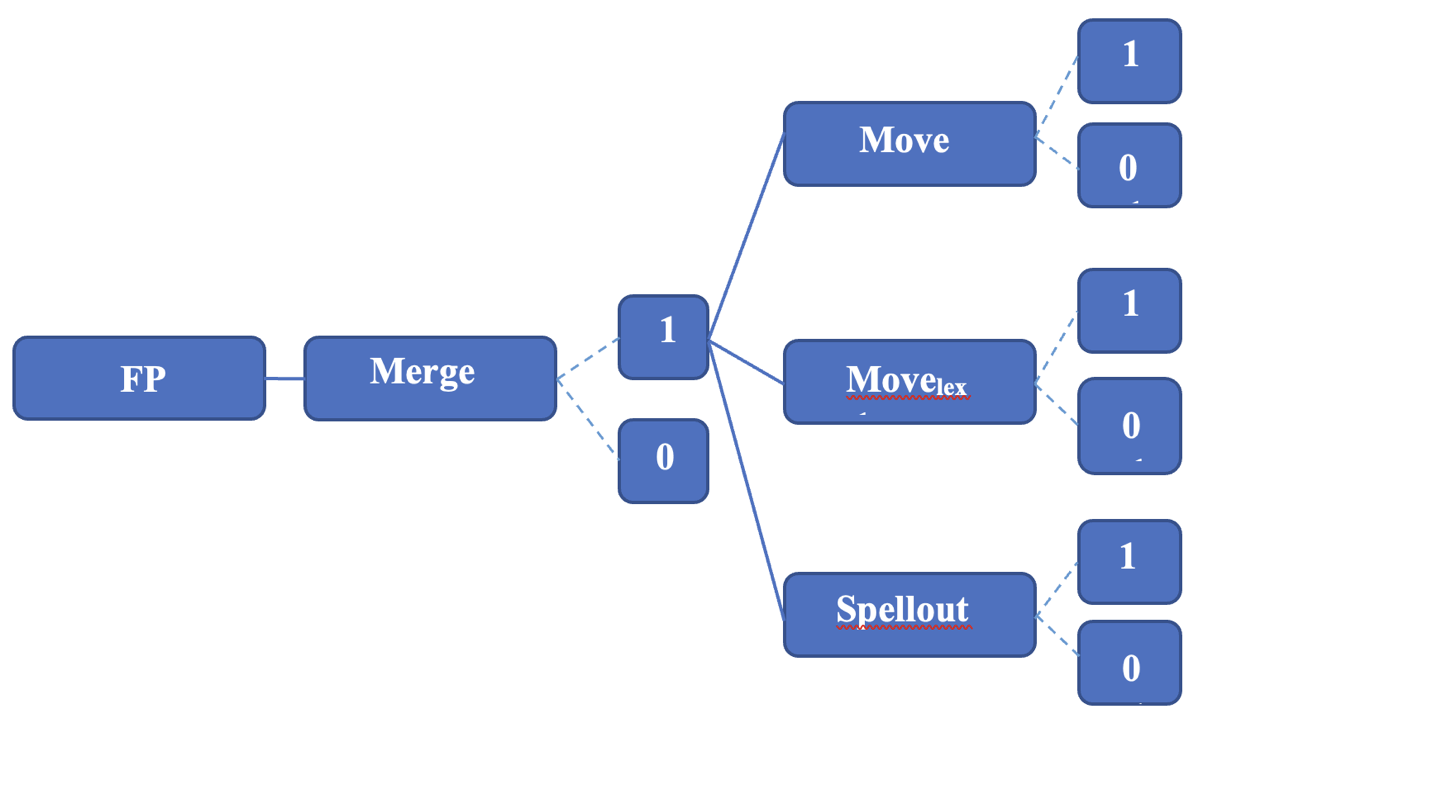
\includegraphics[width=12cm, height=6cm]{images/combinationsfrenchb.png}
    \end{center}

\end{frame}
%=-=-=-=-=-=-=-=-=-=-=-=-=-=-=-=-=-=-=-=-=-=-=-=-=-=-=-=-=-=-=-=-=-=-=-=-=-=-=-=
%   FRAME START   -=-=-=-=-=-=-=-=-=-=-=-=-=-=-=-=-=-=-=-=-=-=-=-=-=-=-=-=-=-=-=
\begin{frame}[c]{Combinations for French}

    \begin{center}
        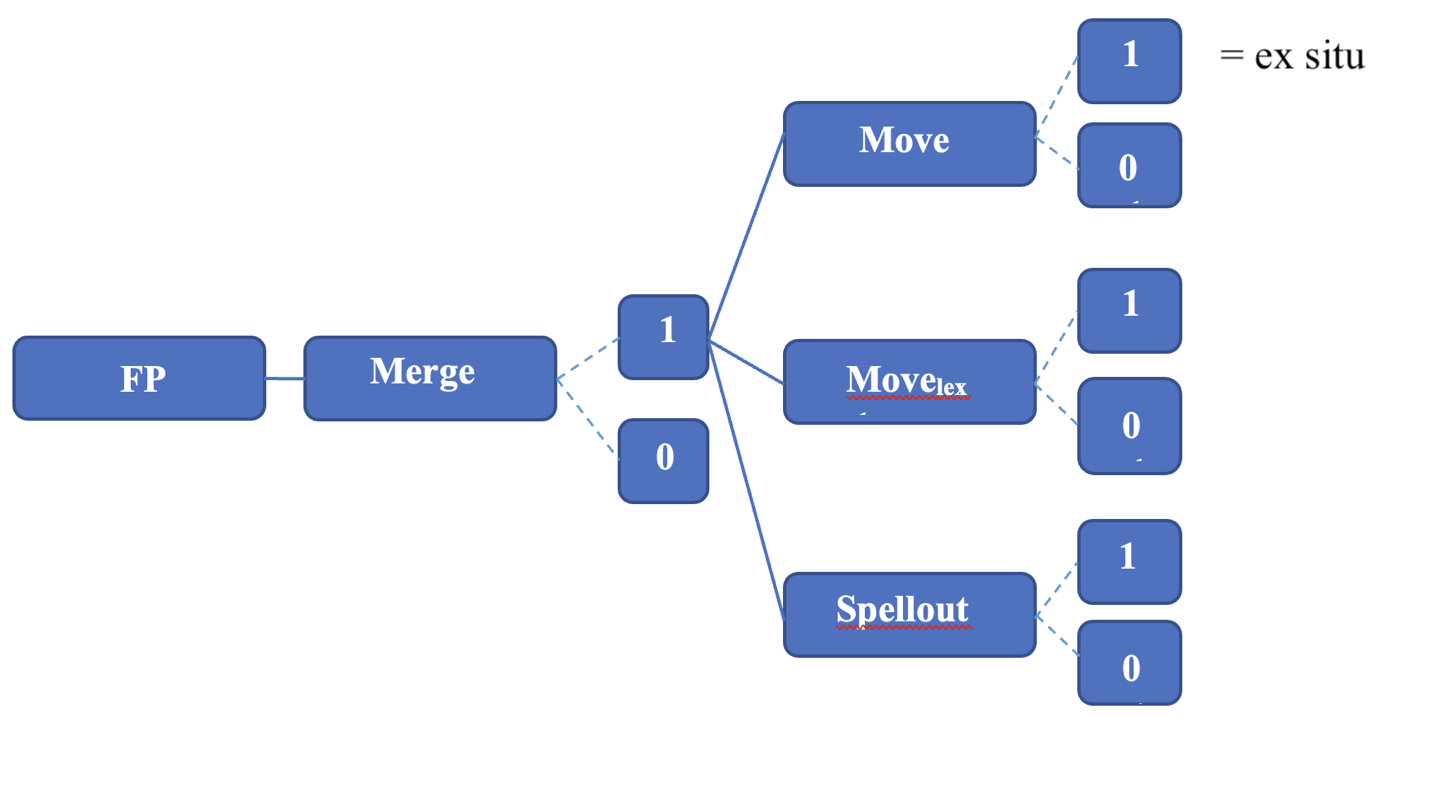
\includegraphics[width=12cm, height=6cm]{images/combinationsfrench1.png}
    \end{center}

\end{frame}
%=-=-=-=-=-=-=-=-=-=-=-=-=-=-=-=-=-=-=-=-=-=-=-=-=-=-=-=-=-=-=-=-=-=-=-=-=-=-=-=
%   FRAME START   -=-=-=-=-=-=-=-=-=-=-=-=-=-=-=-=-=-=-=-=-=-=-=-=-=-=-=-=-=-=-=
\begin{frame}[c]{Combinations for French}

    \begin{center}
        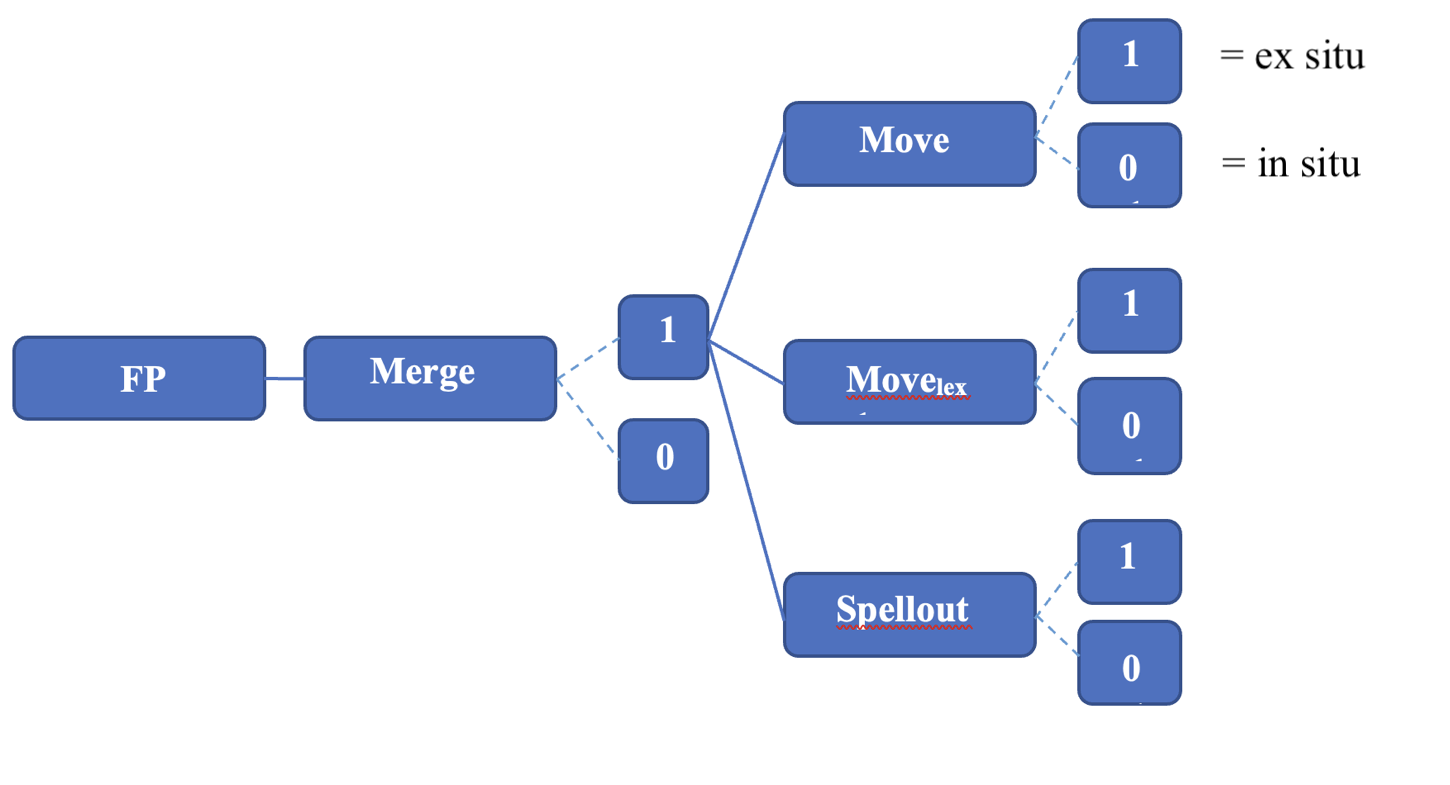
\includegraphics[width=12cm, height=6cm]{images/combinationsfrench2.png}
    \end{center}

\end{frame}
%=-=-=-=-=-=-=-=-=-=-=-=-=-=-=-=-=-=-=-=-=-=-=-=-=-=-=-=-=-=-=-=-=-=-=-=-=-=-=-=
%   FRAME START   -=-=-=-=-=-=-=-=-=-=-=-=-=-=-=-=-=-=-=-=-=-=-=-=-=-=-=-=-=-=-=
\begin{frame}[c]{Combinations for French}

    \begin{center}
        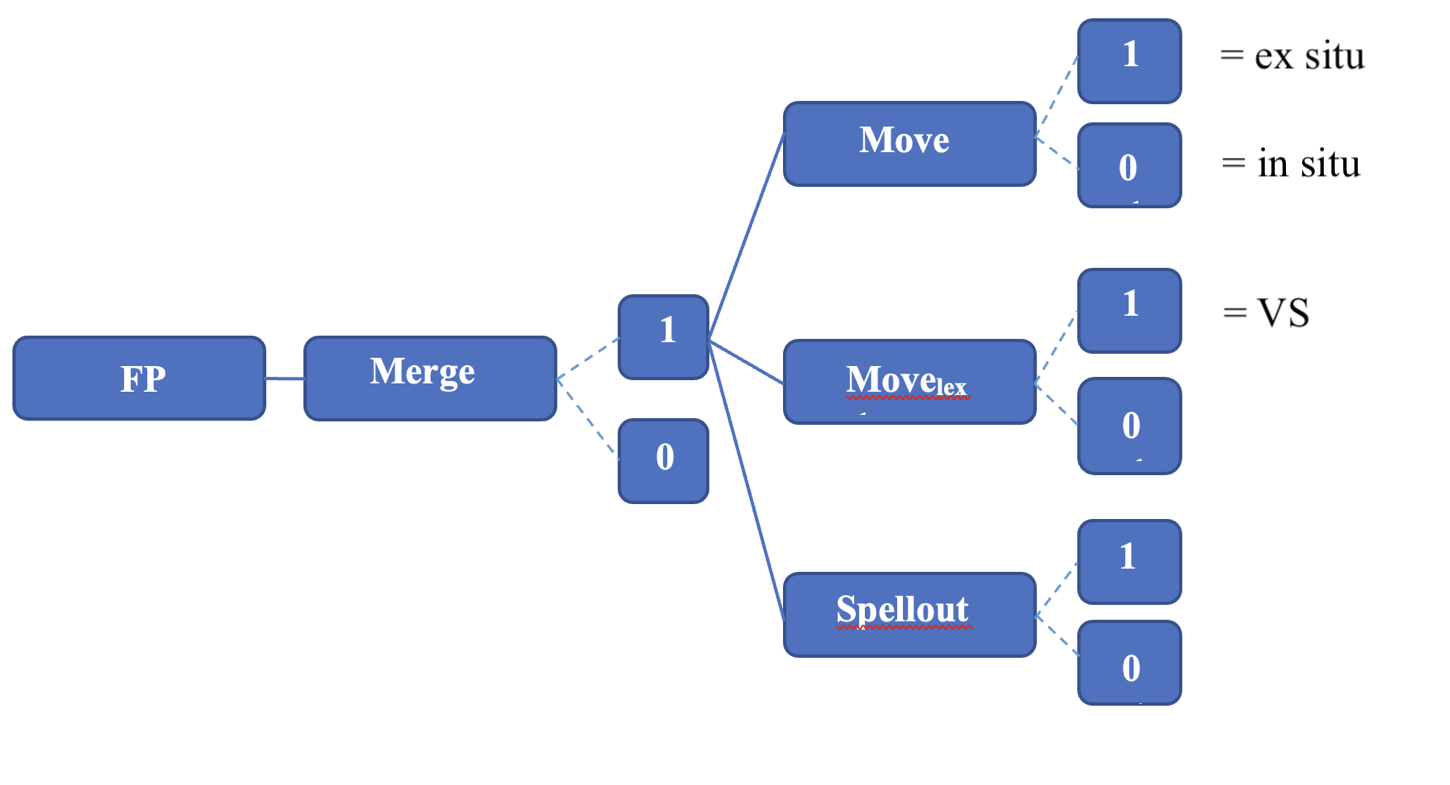
\includegraphics[width=12cm, height=6cm]{images/combinationsfrench3.png}
    \end{center}

\end{frame}
%=-=-=-=-=-=-=-=-=-=-=-=-=-=-=-=-=-=-=-=-=-=-=-=-=-=-=-=-=-=-=-=-=-=-=-=-=-=-=-=
%   FRAME START   -=-=-=-=-=-=-=-=-=-=-=-=-=-=-=-=-=-=-=-=-=-=-=-=-=-=-=-=-=-=-=
\begin{frame}[c]{Combinations for French}

    \begin{center}
        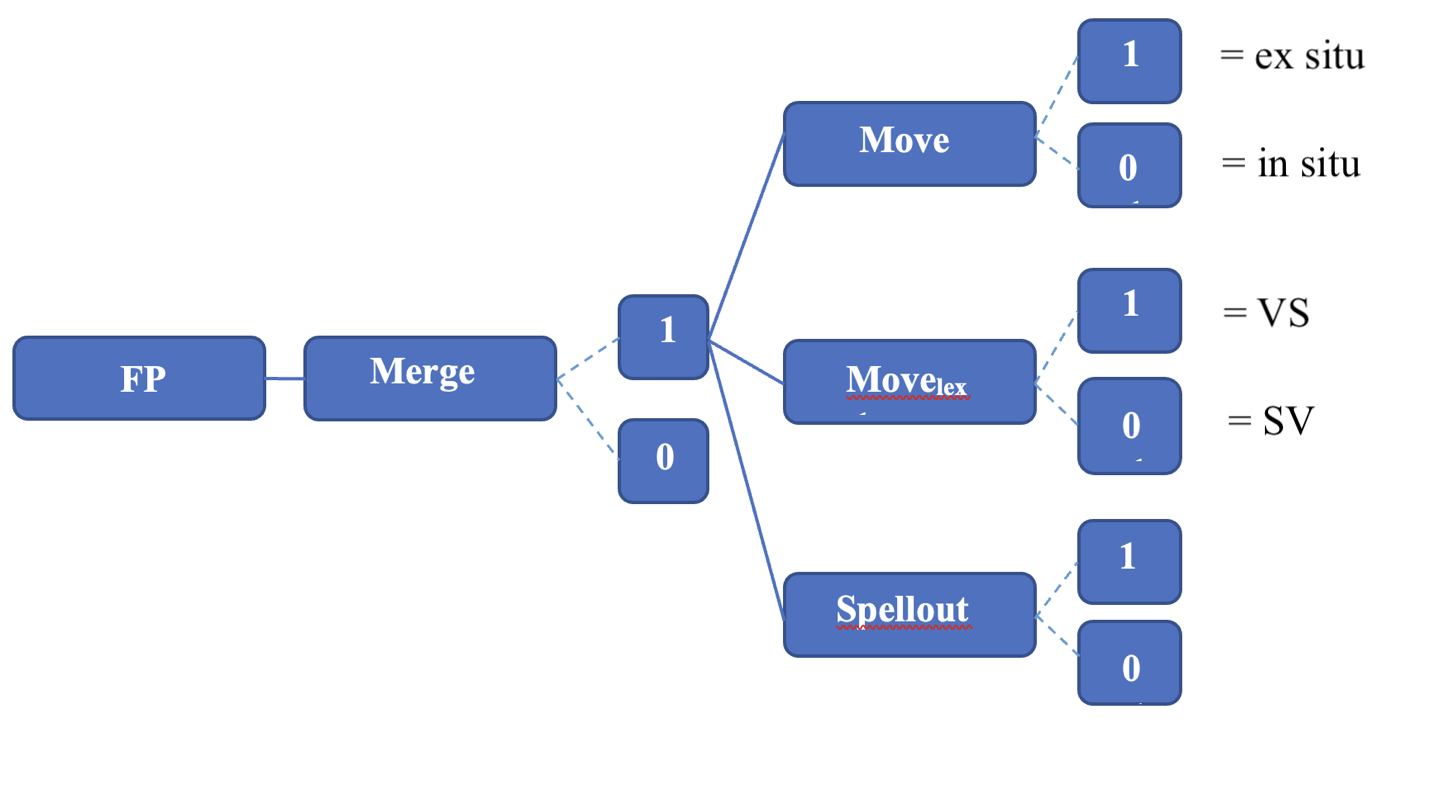
\includegraphics[width=12cm, height=6cm]{images/combinationsfrench4.png}
    \end{center}

\end{frame}
%=-=-=-=-=-=-=-=-=-=-=-=-=-=-=-=-=-=-=-=-=-=-=-=-=-=-=-=-=-=-=-=-=-=-=-=-=-=-=-=
%   FRAME START   -=-=-=-=-=-=-=-=-=-=-=-=-=-=-=-=-=-=-=-=-=-=-=-=-=-=-=-=-=-=-=
\begin{frame}[c]{Combinations for French}

    \begin{center}
        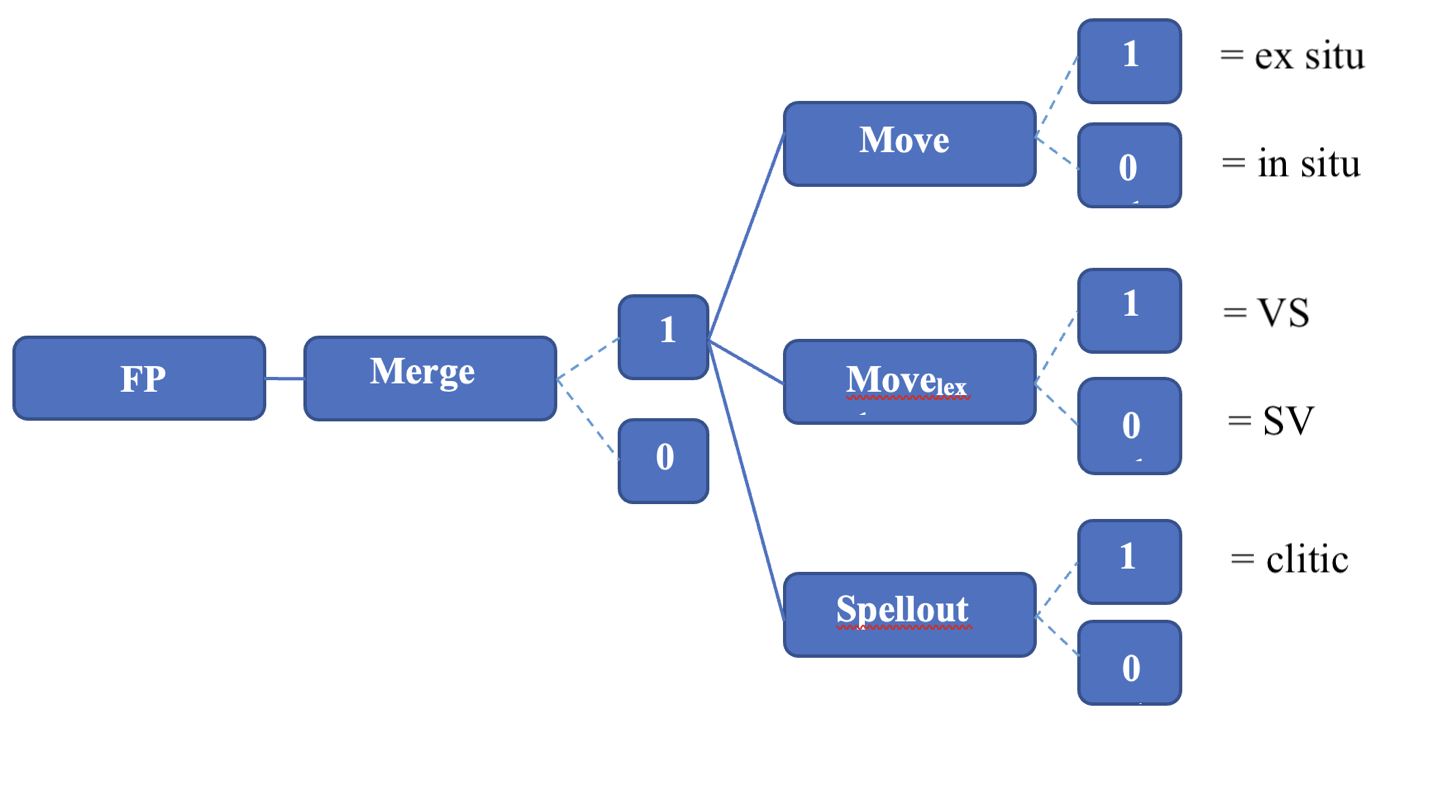
\includegraphics[width=12cm, height=6cm]{images/combinationsfrench5.png}
    \end{center}

\end{frame}
%=-=-=-=-=-=-=-=-=-=-=-=-=-=-=-=-=-=-=-=-=-=-=-=-=-=-=-=-=-=-=-=-=-=-=-=-=-=-=-=
%   FRAME START   -=-=-=-=-=-=-=-=-=-=-=-=-=-=-=-=-=-=-=-=-=-=-=-=-=-=-=-=-=-=-=
\begin{frame}[c]{Combinations for French}

    \begin{center}
        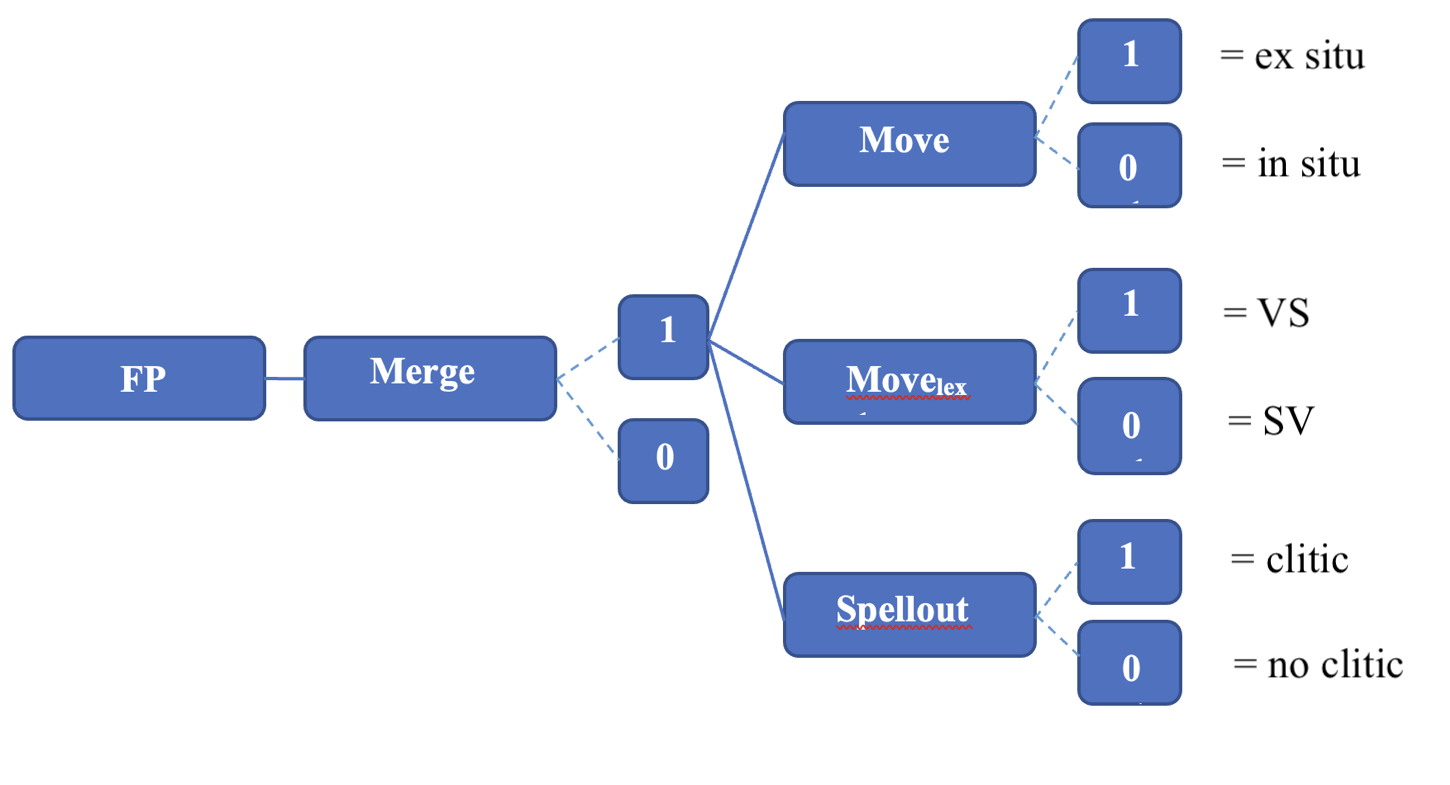
\includegraphics[width=12cm, height=6cm]{images/combinationsfrench6.png}
    \end{center}

\end{frame}
%=-=-=-=-=-=-=-=-=-=-=-=-=-=-=-=-=-=-=-=-=-=-=-=-=-=-=-=-=-=-=-=-=-=-=-=-=-=-=-=
%=-=-=-=-=-=-=-=-=-=-=-=-=-=-=-=-=-=-=-=-=-=-=-=-=-=-=-=-=-=-=-=-=-=-=-=-=-=-=-=
\end{document}